%% start of file `template.tex'.
%% Copyright 2006-2013 Xavier Danaux (xdanaux@gmail.com).
%
% This work may be distributed and/or modified under the
% conditions of the LaTeX Project Public License version 1.3c,
% available at http://www.latex-project.org/lppl/.



\documentclass[11pt,a4paper,sans]{moderncv}        % possible options include font size ('10pt', '11pt' and '12pt'), paper size ('a4paper', 'letterpaper', 'a5paper', 'legalpaper', 'executivepaper' and 'landscape') and font family ('sans' and 'roman')

% moderncv themes
\moderncvstyle{classic}                             % style options are 'casual' (default), 'classic', 'oldstyle' and 'banking'
\moderncvcolor{red}                               % color options 'blue' (default), 'orange', 'green', 'red', 'purple', 'grey' and 'black'
%\renewcommand{\familydefault}{\sfdefault}         % to set the default font; use '\sfdefault' for the default sans serif font, '\rmdefault' for the default roman one, or any tex font name
%\nopagenumbers{}                                  % uncomment to suppress automatic page numbering for CVs longer than one page

% character encoding
\usepackage[utf8]{inputenc}                       % if you are not using xelatex ou lualatex, replace by the encoding you are using
%\usepackage{CJKutf8}                              % if you need to use CJK to typeset your resume in Chinese, Japanese or Korean

% adjust the page margins
\usepackage[top    = 2.75cm,bottom = 2.50cm,left   = 2.50cm,right  = 3.00cm]{geometry}
\setlength{\hintscolumnwidth}{2cm}
\AtBeginDocument{\recomputelengths}
%\setlength{\hintscolumnwidth}{3cm}                % if you want to change the width of the column with the dates
\setlength{\makecvtitlenamewidth}{10cm}           % for the 'classic' style, if you want to force the width allocated to your name and avoid line breaks. be careful though, the length is normally calculated to avoid any overlap with your personal info; use this at your own typographical risks...

\usepackage{wrapfig}

\usepackage{CV_INFO}



% personal data
\firstname{\Huge \GONCVfirstname}
\familyname{\\ \huge \GONCVfamilyname}
%\name{Gonzalo}{Rodr\'iguez Canosa}
\title{\GONCVtitle}               % optional, remove the line if not wanted
\extrainfo{\GONCVextrainfo} 
%\address{Madrid (SPAIN)}{}    % optional, remove the line if not wanted
\address{C/Agustín Durán 30, 1ºIZQ}{28028 Madrid (SPAIN)}    % optional, remove the line if not wanted
\phone[mobile]{+34 617599017}                    % optional, remove the line if not wanted
%\phone{+34 913363010}                      % optional, remove the line if not wanted
%\fax{fax (optional)}                          % optional, remove the line if not wanted
\email{grcanosa@gmail.com}                      % optional, remove the line if not wanted
%\social[linkedin]{grcanosa} 
%\homepage{http://es.linkedin.com/in/grcanosa/en}
\photo[64pt][0pt]{personal_photo.jpg}  





% % personal data
% \name{John}{Doe}
% \title{Resumé title}                               % optional, remove / comment the line if not wanted
% \address{street and number}{postcode city}{country}% optional, remove / comment the line if not wanted; the "postcode city" and "country" arguments can be omitted or provided empty
% \phone[mobile]{+1~(234)~567~890}                   % optional, remove / comment the line if not wanted; the optional "type" of the phone can be "mobile" (default), "fixed" or "fax"
% \phone[fixed]{+2~(345)~678~901}
% \phone[fax]{+3~(456)~789~012}
% \email{john@doe.org}                               % optional, remove / comment the line if not wanted
% \homepage{www.johndoe.com}                         % optional, remove / comment the line if not wanted
% \social[linkedin]{john.doe}                        % optional, remove / comment the line if not wanted
% \social[twitter]{jdoe}                             % optional, remove / comment the line if not wanted
% \social[github]{jdoe}                              % optional, remove / comment the line if not wanted
% \extrainfo{additional information}                 % optional, remove / comment the line if not wanted
% \photo[64pt][0.4pt]{picture}                       % optional, remove / comment the line if not wanted; '64pt' is the height the picture must be resized to, 0.4pt is the thickness of the frame around it (put it to 0pt for no frame) and 'picture' is the name of the picture file
% \quote{Some quote}                                 % optional, remove / comment the line if not wanted

% to show numerical labels in the bibliography (default is to show no labels); only useful if you make citations in your resume
%\makeatletter
%\renewcommand*{\bibliographyitemlabel}{\@biblabel{\arabic{enumiv}}}
%\makeatother
%\renewcommand*{\bibliographyitemlabel}{[\arabic{enumiv}]}% CONSIDER REPLACING THE ABOVE BY THIS

% bibliography with mutiple entries
%\usepackage{multibib}
%\newcites{book,misc}{{Books},{Others}}
%----------------------------------------------------------------------------------
%            content
%----------------------------------------------------------------------------------

\definecolor{color0}{rgb}{0,0,0}% black
\definecolor{color1}{rgb}{0.545098,0,0}% burgundy
%\definecolor{color1}{rgb}{0.2,0.2,0.2}% Testcolor
\definecolor{color2}{rgb}{0.35,0.35,0.35}% dark grey

\quote{\GONCVquote}   


\usepackage{etoolbox}

\patchcmd{\recomputecvlengths}{%
  \setlength{\quotewidth}{0.65\textwidth}%
}{%
  \setlength{\quotewidth}{0.8\textwidth}%
}{}{}

\newtoggle{toggleEXPERTISESECTION}

\usepackage{lastpage}
\rfoot{\textcolor{gray}{\textit{\small{\thepage/\pageref{LastPage}}}}}

\begin{document}

%-----       resume       ---------------------------------------------------------
\makecvtitle

\section{\GONCVsecPROFESIONALEXPERIENCE}
\subsection{\GONCVsecPROFESIONALEXPERIENCEworking}
\GONCVworkingEPROSIMA
\GONCVworkingUPM
\GONCVworkingUOA
\GONCVworkingBOMBARDIER
              % arguments 3 to 6 are optional
\subsection{\GONCVsecPROFESIONALEXPERIENCEscholarships}
\GONCVbecasTRANSPORTES
\GONCVbecasAUTOMATICA

\section{\GONCVsecEDU}
\GONCVeduPHD
\GONCVeduMSC
\GONCVeduERASMUS
\GONCVeduUS
\GONCVeduINSTI
\GONCVeduCOLEGIO



\section{\GONCVsecLANGUAGES}
\GONCVlanSPA
\GONCVlanENG
\GONCVlanGER



\newpage
% \section{Computer skills}
% \cvline{OS}{Windows XP, Vista, Linux (Ubuntu).}
% \cvline{Office}{MS Word, Excel, PowerPoint and LaTeX.}
% \cvline{Programming}{C, C++, Matlab, HTML.}
% \cvline{Simulation}{Webots, Player-Gazebo, Simulink.}
% \cvline{Robotics}{Robot Operating System (ROS), 3D Vision, OpenCV, PCL (Point Cloud Library), OpenGL.}
% %\cvline{Engeeniering}{Advanced Matlab Programming, SolidEdge 3D, AutoCAD 2D-3D.}

\begin{small}

\section{\GONCVsecSKILLS}
\subsection{\GONCVsecCOMPUTER}
\GONCVskillSO
\GONCVskillOFFICE
\GONCVskillCPP
\GONCVskillPROGRAM
\GONCVskillDEVELOP

\subsection{\GONCVsecINGENIERIA}
\GONCVingSIMU
\GONCVingMATLAB
\GONCVingROBOTIC
\GONCVingVISION
\GONCVingHW


\section{\GONCVsecPROJECTS}
\cvline{2011 - 2013}{ROTOS national project. Multirobot Systems for protection of large critical infraestructures. Ref: DPI2010-17998 of DPI subprogram}
\cvline{2009 - 2010}{Networked Multi-Robot Systems (NMRS) project by the European Defense Agency. B-0004-ESM2\_ERG.}

 \section{\GONCVsecPUBLICATIONS}
 \cvline{$\bullet$}{ G. Rodríguez-Canosa, A. Barrientos y J. Cerro \textit{Detection and Tracking of Dynamic
Objects by Using a Multirobot System: Application to Critical Infrastructures Surveillance} Sensors. vol.14 -2 pags. 2911 - 2943. 2014.}
\cvline{$\bullet$}{G. Rodríguez Canosa. \textit{Caracterizaci\'on de Infraestructuras Críticas y su influencia sobre sistemas de seguridad robt\'oticos.} Marzo 2013. \url{http://oa.upm.es/10410/4/CaracteristicasICE_marzo_2013.pdf}}
 \cvline{$\bullet$}{D. Sanz, G. Rodríguez-Canosa, J. Barrientos, J. Cerro, J. Hernandez, A. Barrientos. \textit{Sensorized robotic sphere for large exterior critical infrastructures supervision} Journal of Applied Remote Sensing vol.7 pags. 1-19 (F.I. .876) 2013. JCR: 1.953}
\cvline{$\bullet$}{Gonzalo R. Rodríguez-Canosa, Stephen Thomas, Jaime del Cerro, Antonio Barrientos and Bruce MacDonald.\textit{A Real-Time Method to Detect and Track Moving Objects (DATMO) from Unmanned Aerial Vehicles (UAVs) Using a Single Camera}. Remote Sensensing. 2012, 4(4), 1090-1111; doi:10.3390/rs4041090. JCR: 2.171}
% \cvline{$\bullet$}{Gonzalo R. Rodríguez-Canosa, J.Del Cerro and A. Barrientos. \textit{Detección e Identificación de Objetos Móviles en Sistemas Multi-Robot con Información 3D}. 8th Workshop of Robocity 2030-II on Exterior Robots. Madrid, November 2010.}

\section{\GONCVsecTESIS}
\GONCVtesisINFO
\GONCVtesisDESCRIPTION

\end{small}


\GONCVuseEXPERTISESECTION

\iftoggle{toggleEXPERTISESECTION}
{

\begin{small}

\section{\GONCVsecPREVIOUSEXPERIENCE}

\subsection{\GONCVpreviousRTPS}
\GONCVpreviousRTPSdescription

\subsection{\GONCVpreviousROTOS}
\begin{wrapfigure}{l}{0.25\textwidth}
\vspace{-0.3cm}
\centering
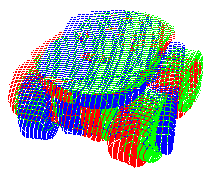
\includegraphics[width=0.24\textwidth]{svd_sac_ia_sac_better.png}
\vspace{-0.3cm}
\end{wrapfigure}
\GONCVpreviousROTOSdescription

\subsection{\GONCVpreviousUAVAUCKLAND}
\begin{wrapfigure}{l}{0.25\textwidth}
\vspace{-0.3cm}
\centering
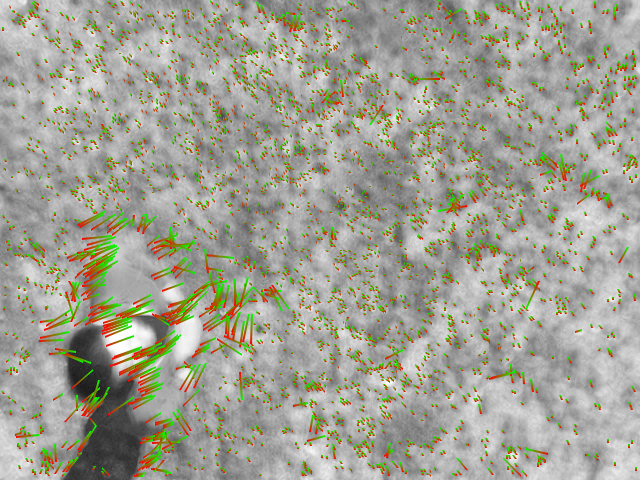
\includegraphics[width=0.24\textwidth]{r1_realoptflow.png}
\vspace{-0.3cm}
\end{wrapfigure}
\GONCVpreviousUAVAUCKLANDdescription


\subsection{\GONCVpreviousUPMDATMO}
\begin{wrapfigure}{l}{0.25\textwidth}
\vspace{-0.3cm}
\centering
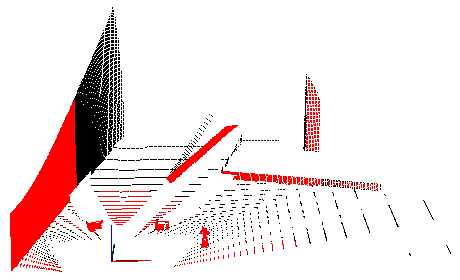
\includegraphics[width=0.24\textwidth]{pcpre_isolated_points.png}
\vspace{0.2cm}
\end{wrapfigure}
\GONCVpreviousUPMDATMOdescription

\subsection{\GONCVpreviousBOMBARDIER}
\GONCVpreviousBOMBARDIERdescription

\subsection{\GONCVpreviousCANBUS}
\GONCVpreviousCANBUSdescription

\subsection{\GONCVpreviousTRANSPORTES}
\begin{wrapfigure}{l}{0.25\textwidth}
\vspace{-0.3cm}
\centering
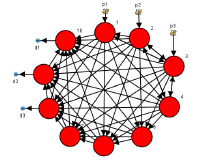
\includegraphics[width=0.24\textwidth]{redtopo.png}
\vspace{-0.3cm}
\end{wrapfigure}
\GONCVpreviousTRANSPORTESdescription

\end{small}
}
{
}




% \section{Extra Curricular Activities}
% \cvline{July 2012}{Cooperation of Robots and Sensor Networks. GKmM Summer School 2012.\newline \url{http://www.gkmm.tu-darmstadt.de/summerschool/?q=node/1}}
% \cvline{2011}{Organization of \textit{Cybertech 2011} contest. The contest objective is to build and program a robot able to follow a line; passing by other vehicles and avoiding obstacles; and also find the exit through a maze. Organizing the contest involves teaching three courses to the participants and supervise the developments of some of the groups, providing support.}
% \cvline{Sept. 2010}{Participation in CEABOT 2010 contest. Humanoid robots contest with three main tests: a) walking avoiding obstacles, b) stairs climbing, and c) sumo fights with other robots. 4th place out of 11 groups from Spanish universities.}
% \cvline{Nov. 2010}{Participation and oral presentation in 8th Workshop of Robocity 2030-II on Exterior Robots in Automatic and Robotic Center (CAR) in Madrid.}
% \cvline{2007}{Signals, Sensors and Systems Seminar in KTH, Stockholm.}
% 
% \section{Awards and Memberships}
% \cvline{2011}{Student Member of IEEE}
% \cvline{2010}{Student Member of CEA-IFAC - Comité Español de Automática (Spanish Automation Committee).}
% \cvline{2010}{Student Member of Robocity 2030-II Robotics Consortium.}
% \cvline{2002}{Secondary Education with Honors by Junta de Andalucía, Spain.}


% 
% \section{Education}
% \cventry{year--year}{Degree}{Institution}{City}{\textit{Grade}}{Description}  % arguments 3 to 6 can be left empty
% \cventry{year--year}{Degree}{Institution}{City}{\textit{Grade}}{Description}
% 
% \section{Master thesis}
% \cvitem{title}{\emph{Title}}
% \cvitem{supervisors}{Supervisors}
% \cvitem{description}{Short thesis abstract}
% 
% \section{Experience}
% \subsection{Vocational}
% \cventry{year--year}{Job title}{Employer}{City}{}{General description no longer than 1--2 lines.\newline{}%
% Detailed achievements:%
% \begin{itemize}%
% \item Achievement 1;
% \item Achievement 2, with sub-achievements:
%   \begin{itemize}%
%   \item Sub-achievement (a);
%   \item Sub-achievement (b), with sub-sub-achievements (don't do this!);
%     \begin{itemize}
%     \item Sub-sub-achievement i;
%     \item Sub-sub-achievement ii;
%     \item Sub-sub-achievement iii;
%     \end{itemize}
%   \item Sub-achievement (c);
%   \end{itemize}
% \item Achievement 3.
% \end{itemize}}
% \cventry{year--year}{Job title}{Employer}{City}{}{Description line 1\newline{}Description line 2}
% \subsection{Miscellaneous}
% \cventry{year--year}{Job title}{Employer}{City}{}{Description}
% 
% \section{Languages}
% \cvitemwithcomment{Language 1}{Skill level}{Comment}
% \cvitemwithcomment{Language 2}{Skill level}{Comment}
% \cvitemwithcomment{Language 3}{Skill level}{Comment}
% 
% \section{Computer skills}
% \cvdoubleitem{category 1}{XXX, YYY, ZZZ}{category 4}{XXX, YYY, ZZZ}
% \cvdoubleitem{category 2}{XXX, YYY, ZZZ}{category 5}{XXX, YYY, ZZZ}
% \cvdoubleitem{category 3}{XXX, YYY, ZZZ}{category 6}{XXX, YYY, ZZZ}
% 
% \section{Interests}
% \cvitem{hobby 1}{Description}
% \cvitem{hobby 2}{Description}
% \cvitem{hobby 3}{Description}
% 
% \section{Extra 1}
% \cvlistitem{Item 1}
% \cvlistitem{Item 2}
% \cvlistitem{Item 3. This item is particularly long and therefore normally spans over several lines. Did you notice the indentation when the line wraps?}
% 
% \section{Extra 2}
% \cvlistdoubleitem{Item 1}{Item 4}
% \cvlistdoubleitem{Item 2}{Item 5\cite{book1}}
% \cvlistdoubleitem{Item 3}{Item 6. Like item 3 in the single column list before, this item is particularly long to wrap over several lines.}
% 
% \section{References}
% \begin{cvcolumns}
%   \cvcolumn{Category 1}{\begin{itemize}\item Person 1\item Person 2\item Person 3\end{itemize}}
%   \cvcolumn{Category 2}{Amongst others:\begin{itemize}\item Person 1, and\item Person 2\end{itemize}(more upon request)}
%   \cvcolumn[0.5]{All the rest \& some more}{\textit{That} person, and \textbf{those} also (all available upon request).}
% \end{cvcolumns}
% 
% % Publications from a BibTeX file without multibib
% %  for numerical labels: \renewcommand{\bibliographyitemlabel}{\@biblabel{\arabic{enumiv}}}% CONSIDER MERGING WITH PREAMBLE PART
% %  to redefine the heading string ("Publications"): \renewcommand{\refname}{Articles}
% \nocite{*}
% \bibliographystyle{plain}
% \bibliography{publications}                        % 'publications' is the name of a BibTeX file

% Publications from a BibTeX file using the multibib package
%\section{Publications}
%\nocitebook{book1,book2}
%\bibliographystylebook{plain}
%\bibliographybook{publications}                   % 'publications' is the name of a BibTeX file
%\nocitemisc{misc1,misc2,misc3}
%\bibliographystylemisc{plain}
%\bibliographymisc{publications}                   % 'publications' is the name of a BibTeX file

% \clearpage
% %-----       letter       ---------------------------------------------------------
% % recipient data
% \recipient{Company Recruitment team}{Company, Inc.\\123 somestreet\\some city}
% \date{January 01, 1984}
% \opening{Dear Sir or Madam,}
% \closing{Yours faithfully,}
% \enclosure[Attached]{curriculum vit\ae{}}          % use an optional argument to use a string other than "Enclosure", or redefine \enclname
% \makelettertitle
% 
% Lorem ipsum dolor sit amet, consectetur adipiscing elit. Duis ullamcorper neque sit amet lectus facilisis sed luctus nisl iaculis. Vivamus at neque arcu, sed tempor quam. Curabitur pharetra tincidunt tincidunt. Morbi volutpat feugiat mauris, quis tempor neque vehicula volutpat. Duis tristique justo vel massa fermentum accumsan. Mauris ante elit, feugiat vestibulum tempor eget, eleifend ac ipsum. Donec scelerisque lobortis ipsum eu vestibulum. Pellentesque vel massa at felis accumsan rhoncus.
% 
% Suspendisse commodo, massa eu congue tincidunt, elit mauris pellentesque orci, cursus tempor odio nisl euismod augue. Aliquam adipiscing nibh ut odio sodales et pulvinar tortor laoreet. Mauris a accumsan ligula. Class aptent taciti sociosqu ad litora torquent per conubia nostra, per inceptos himenaeos. Suspendisse vulputate sem vehicula ipsum varius nec tempus dui dapibus. Phasellus et est urna, ut auctor erat. Sed tincidunt odio id odio aliquam mattis. Donec sapien nulla, feugiat eget adipiscing sit amet, lacinia ut dolor. Phasellus tincidunt, leo a fringilla consectetur, felis diam aliquam urna, vitae aliquet lectus orci nec velit. Vivamus dapibus varius blandit.
% 
% Duis sit amet magna ante, at sodales diam. Aenean consectetur porta risus et sagittis. Ut interdum, enim varius pellentesque tincidunt, magna libero sodales tortor, ut fermentum nunc metus a ante. Vivamus odio leo, tincidunt eu luctus ut, sollicitudin sit amet metus. Nunc sed orci lectus. Ut sodales magna sed velit volutpat sit amet pulvinar diam venenatis.
% 
% Albert Einstein discovered that $e=mc^2$ in 1905.
% 
% \[ e=\lim_{n \to \infty} \left(1+\frac{1}{n}\right)^n \]
% 
% \makeletterclosing

%\clearpage\end{CJK*}                              % if you are typesetting your resume in Chinese using CJK; the \clearpage is required for fancyhdr to work correctly with CJK, though it kills the page numbering by making \lastpage undefined
\end{document}


%% end of file `template.tex'.
